\documentclass[journal,12pt,twocolumn]{IEEEtran}

\usepackage{setspace}
\usepackage{gensymb}

\singlespacing


\usepackage[cmex10]{amsmath}

\usepackage{amsthm}

\usepackage{mathrsfs}
\usepackage{txfonts}
\usepackage{stfloats}
\usepackage{bm}
\usepackage{cite}
\usepackage{cases}
\usepackage{blkarray}

\usepackage{longtable}
\usepackage{multirow}

\usepackage{enumitem}
\usepackage{mathtools}
\usepackage{steinmetz}
\usepackage{tikz}
\usepackage{circuitikz}
\usepackage{verbatim}
\usepackage{tfrupee}
\usepackage[breaklinks=true]{hyperref}
\usepackage{graphicx}
\usepackage{graphics}
\usepackage{tkz-euclide}
\usepackage{float}
\usepackage{caption}
\usepackage{subcaption}

\usetikzlibrary{calc,math}
\usetikzlibrary{arrows,automata}
\usepackage{listings}
    \usepackage{color}                                            %%
    \usepackage{array}                                            %%
    \usepackage{longtable}                                        %%
    \usepackage{calc}                                             %%
    \usepackage{multirow}                                         %%
    \usepackage{hhline}                                           %%
    \usepackage{ifthen}                                           %%
    \usepackage{lscape}     
\usepackage{multicol}
\usepackage{chngcntr}

\DeclareMathOperator*{\Res}{Res}

\renewcommand\thesection{\arabic{section}}
\renewcommand\thesubsection{\thesection.\arabic{subsection}}
\renewcommand\thesubsubsection{\thesubsection.\arabic{subsubsection}}

\renewcommand\thesectiondis{\arabic{section}}
\renewcommand\thesubsectiondis{\thesectiondis.\arabic{subsection}}
\renewcommand\thesubsubsectiondis{\thesubsectiondis.\arabic{subsubsection}}


\hyphenation{op-tical net-works semi-conduc-tor}
\def\inputGnumericTable{}                                 %%

\lstset{
%language=C,
frame=single, 
breaklines=true,
columns=fullflexible
}
\begin{document}


\newtheorem{theorem}{Theorem}[section]
\newtheorem{problem}{Problem}
\newtheorem{proposition}{Proposition}[section]
\newtheorem{lemma}{Lemma}[section]
\newtheorem{corollary}[theorem]{Corollary}
\newtheorem{example}{Example}[section]
\newtheorem{definition}[problem]{Definition}

\newcommand{\BEQA}{\begin{eqnarray}}
\newcommand{\EEQA}{\end{eqnarray}}
\newcommand{\define}{\stackrel{\triangle}{=}}
\newcommand\hlight[1]{\tikz[overlay, remember picture,baseline=-\the\dimexpr\fontdimen22\textfont2\relax]\node[rectangle,fill=blue!50,rounded corners,fill opacity = 0.2,draw,thick,text opacity =1] {$#1$};}
\bibliographystyle{IEEEtran}
\providecommand{\mbf}{\mathbf}
\providecommand{\pr}[1]{\ensuremath{\Pr\left(#1\right)}}
\providecommand{\qfunc}[1]{\ensuremath{Q\left(#1\right)}}
\providecommand{\sbrak}[1]{\ensuremath{{}\left[#1\right]}}
\providecommand{\lsbrak}[1]{\ensuremath{{}\left[#1\right.}}
\providecommand{\rsbrak}[1]{\ensuremath{{}\left.#1\right]}}
\providecommand{\brak}[1]{\ensuremath{\left(#1\right)}}
\providecommand{\lbrak}[1]{\ensuremath{\left(#1\right.}}
\providecommand{\rbrak}[1]{\ensuremath{\left.#1\right)}}
\providecommand{\cbrak}[1]{\ensuremath{\left\{#1\right\}}}
\providecommand{\lcbrak}[1]{\ensuremath{\left\{#1\right.}}
\providecommand{\rcbrak}[1]{\ensuremath{\left.#1\right\}}}
\theoremstyle{remark}
\newtheorem{rem}{Remark}
\newcommand{\sgn}{\mathop{\mathrm{sgn}}}
\providecommand{\abs}[1]{\left\vert#1\right\vert}
\providecommand{\res}[1]{\Res\displaylimits_{#1}} 
\providecommand{\norm}[1]{\left\lVert#1\right\rVert}
%\providecommand{\norm}[1]{\lVert#1\rVert}
\providecommand{\mtx}[1]{\mathbf{#1}}
\providecommand{\mean}[1]{E\left[ #1 \right]}
\providecommand{\fourier}{\overset{\mathcal{F}}{ \rightleftharpoons}}
%\providecommand{\hilbert}{\overset{\mathcal{H}}{ \rightleftharpoons}}
\providecommand{\system}{\overset{\mathcal{H}}{ \longleftrightarrow}}
	%\newcommand{\solution}[2]{\textbf{Solution:}{#1}}
\newcommand{\solution}{\noindent \textbf{Solution: }}
\newcommand{\cosec}{\,\text{cosec}\,}
\providecommand{\dec}[2]{\ensuremath{\overset{#1}{\underset{#2}{\gtrless}}}}
\newcommand{\myvec}[1]{\ensuremath{\begin{pmatrix}#1\end{pmatrix}}}
\newcommand{\mydet}[1]{\ensuremath{\begin{vmatrix}#1\end{vmatrix}}}
\numberwithin{equation}{subsection}
\makeatletter
\@addtoreset{figure}{problem}
\makeatother
\let\StandardTheFigure\thefigure
\let\vec\mathbf
\renewcommand{\thefigure}{\theproblem}
\def\putbox#1#2#3{\makebox[0in][l]{\makebox[#1][l]{}\raisebox{\baselineskip}[0in][0in]{\raisebox{#2}[0in][0in]{#3}}}}
     \def\rightbox#1{\makebox[0in][r]{#1}}
     \def\centbox#1{\makebox[0in]{#1}}
     \def\topbox#1{\raisebox{-\baselineskip}[0in][0in]{#1}}
     \def\midbox#1{\raisebox{-0.5\baselineskip}[0in][0in]{#1}}
\vspace{3cm}
\title{Assignment 18}
\author{K.A. Raja Babu}
\maketitle
\newpage
\bigskip
\renewcommand{\thefigure}{\theenumi}
\renewcommand{\thetable}{\theenumi}
Download all python codes from 
\begin{lstlisting}
https://github.com/ka-raja-babu/Matrix-Theory/tree/main/Assignment18
\end{lstlisting}
%
and latex-tikz codes from 
%
\begin{lstlisting}
https://github.com/ka-raja-babu/Matrix-Theory/tree/main/Assignment18
\end{lstlisting}
%
\section{Question No. 14.8(Markov Chain)}

Consider a simple symmetric random walk on integers, where from every state $i$ you move to $i-1$ and $i+1$ with the probability half each. Then which of the following are true?

\begin{enumerate}
\item The random walk is aperiodic
\item The random walk is irreducible
\item The random walk is null recurrent
\item The random walk is positive recurrent
\end{enumerate}

\section{Solution}

\begin{definition}[Aperiodicity]
A random walk defined by a Markov chain having state space $S$ and state transition matrix $P$ ,is said to be aperiodic if there exists self-transition in the chain such that
\begin{align}
    p^n_{ii}>0 \quad \text{for} \quad i \in S,n \in Z^+
\end{align}
\end{definition}

\begin{definition}[Irreducibility]
A random walk defined by a Markov chain having state space $S$ and state transition matrix $P$ ,is said to be irreducible if all states communicate with each other such that
\begin{align}
    p^n_{ij}>0 \quad \text{for} \quad i,j \in S,n \in Z^+
\end{align}
\end{definition}

\begin{definition}[Positive and Null Recuurancy]
A random walk defined by a Markov chain having state space $S$ ,is said to be positive recurrent if the excepted time to return to state $i$ $\forall$ $i \in S$ is finite such that
\begin{align}
    E(\tau_{ii}) < \infty
\end{align}

and,is said to be null recurrent if the excepted time to return to state $i$ $\forall$ $i \in S$ is infinite such that
\begin{align}
    E(\tau_{ii}) = \infty
\end{align}
\end{definition}

Let us define a Markov Chain for the given simple symmetric random walk with states $\cbrak{i-1,i,i+1}$ .

\begin{figure}[h]
\caption*{\textbf{Markov chain diagram}}
\centering
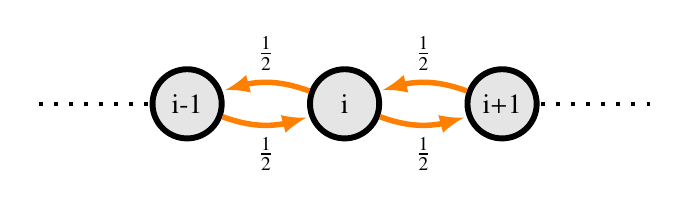
\begin{tikzpicture}
    % Setup the style for the states
        \tikzset{node style/.style={state, 
                                    minimum width=0.2cm,
                                    line width=0.75mm,
                                    fill=gray!20!white}}
        % Draw the states
        \node[node style] at (0,0)      (state_i)   {i};     
        \node[node style] at (2,0)      (state_i+1) {i+1};      
        \node[node style] at (-2,0)     (state_i-1) {i-1};  
        %\node[node style] at (4, 0)     (state_i+2) {i+2}; 
        %\node[node style] at (-4, 0)    (state_i-2) {i-2};
        \draw[line width =0.5mm,loosely dotted] (2.5,0) -- (4,0);
        \draw[line width =0.5mm,loosely dotted] (-2.5,0) -- (-4,0);
        % Connect the states with arrows
        \draw[every loop,
              auto=right,
              line width=0.7mm,
              >=latex,
              draw=orange,
              fill=orange]
        (state_i) edge[bend right = 20] node{$\frac{1}{2}$} (state_i+1)
        (state_i+1) edge[bend right = 20] node{$\frac{1}{2}$} (state_i)
        (state_i) edge[bend right = 20] node{$\frac{1}{2}$}  (state_i-1)
        (state_i-1) edge[bend right = 20] node{$\frac{1}{2}$}  (state_i);
\end{tikzpicture}
\end{figure}

State transition matrix $P$ can be defined as:
\begin{align}
\label{cs2015-291}
    P=\begin{blockarray}{cccc}
& i-1 & i & i+1 \\
\begin{block}{c[ccc]}
  i-1 & 0 & \frac{1}{2}  & \frac{1}{4}  \\
  i & \frac{1}{2} & 0 & \frac{1}{2} \\
  i+1 & \frac{1}{4} & \frac{1}{2} & 0 \\
\end{block}
\end{blockarray}
\end{align}

\begin{enumerate}
    \item From State Transition Matrix $P$,
      \begin{align}
        p_{mm} = 0
    \end{align}
    where
    \begin{align}
        m=\{i-1,i,i+1\} 
    \end{align}
    
    $\because$ There is no self-transition in the chain.
    
    $\therefore$ Random Walk is not aperiodic.

    \item From State Transition Matrix $P$,
    \begin{align}
        p_{mn} > 0  
    \end{align}
    where
    \begin{align}
        m,n=\{i-1,i,i+1\} 
    \end{align}
     
    $\because$ All states communicate with each other .

    $\therefore$ Random Walk is irreducible.

    \item Let $p=\frac{1}{2}$ be the probability to move from state $i$ to state $i+1$ and $q=\frac{1}{2}$ be the probability to move from state $i$ to state $i-1$ .

    Then,the excepted time of getting back to $i$ $\forall$ $i$ is given by 
    \begin{align}
       E(\tau_{ii}) &= \frac{1}{|p-q|} \\
       &=\frac{1}{0} \\
       &= \infty
    \end{align}

    $\therefore$ Random Walk is null recurrent .

\end{enumerate}

Hence, \boxed{Options \quad (2),(3)} are true .

\numberwithin{figure}{section}
\begin{figure}[!ht]
\centering
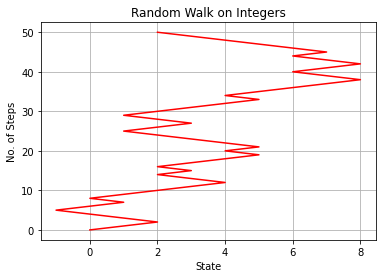
\includegraphics[width=\columnwidth]{Figure18}
\caption{Random Walk on Integers}
\label{Random Walk}	
\end{figure}

\end{document}


